\documentclass[]{report}


\usepackage{blindtext}
\usepackage{titlepic}
\usepackage{titlesec}
\usepackage{graphicx}
\usepackage{float}
\usepackage{titlesec}
\usepackage{listings}
\usepackage[%  
colorlinks=true,
pdfborder={0 0 0},
linkcolor=red
]{hyperref}

\makeatletter
\renewcommand{\@makechapterhead}[1]{%
	\vspace*{50 pt}%
	{\setlength{\parindent}{0pt} \raggedright \normalfont
		\bfseries\Huge
		
		#1\par\nobreak\vspace{40 pt}}}
\makeatother

% Title Page
\title{COSC 3P98 Assignment 3}
\author{Brett Terpstra - 6920201 - bt19ex@brocku.ca}
\titlepic{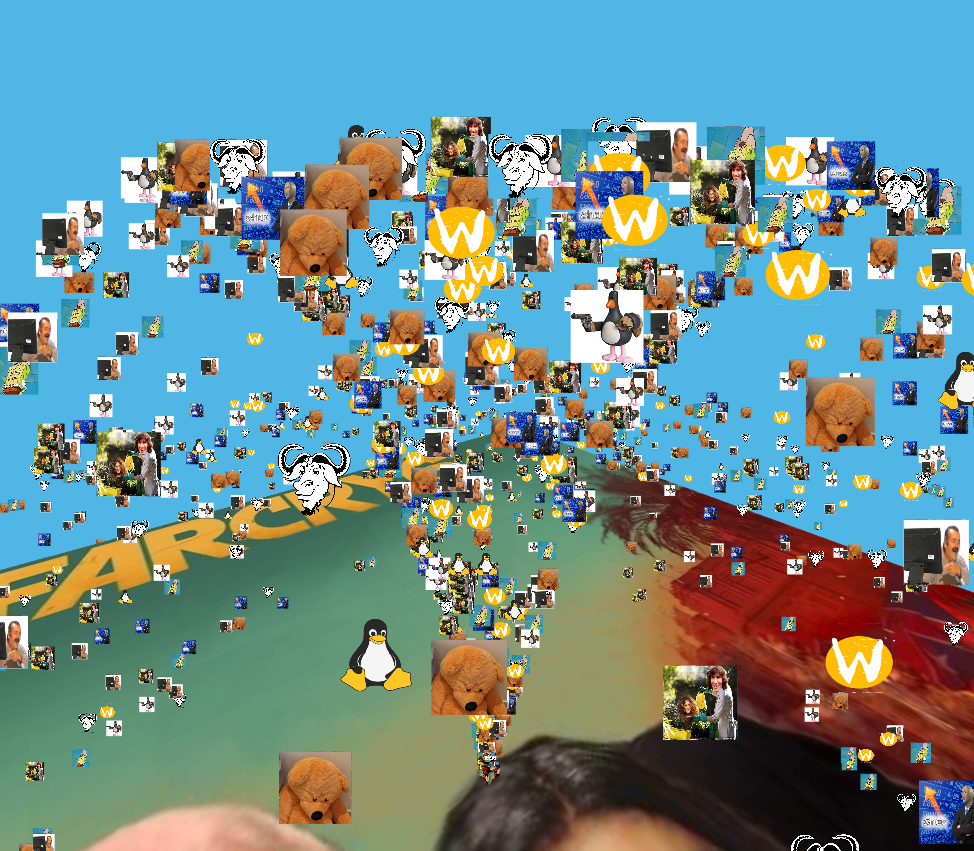
\includegraphics[width=\textwidth]{screenshot001.png}}
\renewcommand*\contentsname{Table Of Contents}



\begin{document}
\maketitle

\begin{abstract}
Particle systems are the cornerstone of all modern game engines as they allow effects such as smoke which are otherwise impossible with static meshes. Ergo a good particle system should be flexible while maintaining stable performance. This document serves as an informal report on the design and implementation of two distinct particle systems; a basic but flexible engine and a high-performance extendable "modern" GPU-powered particle system.
\end{abstract}

\tableofcontents

\chapter{Introduction}
\section{Description}
Over the course of working on this assignment I began to wonder how far I could push my hardware and \autoref{chap:hp} "Performance Mode" will go further into this. As for the main assignment requirements, they are met simply by running the CMake project. On my hardware, the simple particle fountain can reach 30k particles and features sorted transparency.
\subsection{Extra Features}
\begin{itemize}
	\item Ordered Alpha Blending
	\item "Spray" Mode (12)
	\item Textured Particles/Plane/Cube (16)
	\item Particles with Different Textures (18)
	\item Extra Feature - "Performance Mode" (23)
\end{itemize}
\subsection{Missing Features}
The random spin mode was left out intentionally for two reasons. One, I specifically designed the particle structure to fit in 32 bytes, half the width of a cache line. Two, the potential marks were not worth disturbing the particle data structure and further altering the particle system. There is likely little benefit to ensuring the particles fit nicely inside a cache line as most of the CPU time is spent on OpenGL API calls. See \autoref{chap:hp} "Performance Mode" for more information.
\section{Building}
As of writing this report, I have yet to build and test on Windows. The Visual Studio project will build without issues, however, since this assignment was primarily designed and tested on Debian 12 "Bookworm" (Linux 6.1.0-6-amd64) using AMD/Intel hardware (Mesa 22.3.6), I recommend using CMake. 
\subsection{Caveats}
The assignment makes use of a non-standard OpenGL extension during texture loading. "GL\_TEXTURE\_MAX\_ANISOTROPY\_EXT" should work on all modern Intel/AMD/Nvidia hardware, if it doesn't work on your hardware consider removing the line from texture.h and high\_perf.cpp
\subsection{Build Commands}
\begin{figure}[H]
	\centering
	\begin{verbatim}
	mkdir build && cd build
	cmake -DCMAKE_BUILD_TYPE=Release ../
	make -j 16
	./assign3
	\end{verbatim}
	\caption{Linux build commands.}
\end{figure}
\section{Usage}
Keybindings and usage instructions are printed at program startup.

\chapter{Performance Mode}\label{chap:hp}
\section{Design}
The high-performance mode is the result of a weekend hack-a-ton where I wanted to see how easy it would be to implement a million particle+ renderer. If I had more time I would encapsulate the high\_perf.cpp file into the particle system class, allowing for multiple *and customizable* particle systems. If you wish to change settings, most are constants in shaders/physics.comp or high\_perf/high\_perf.cpp. The rendering engine itself can handle around 20 million particles at about 60fps (\autoref{fig:screenshot002}). With physics enabled, the engine can handle about 6 million particles (\autoref{fig:phyiscsrend}) but as \autoref{fig:phyiscsrendfill} shows, the renderer is fillrate limited. Solutions to increase the number of rendered particles are discussed in \autoref{sec:fp}. It should be noted that (\autoref{fig:screenshot002}) used a previous renderer that made use of an instanced "GL\_TRIANGLES" approach and did not have textures or billboarding. The new renderer (\autoref{fig:newrender}) makes use of "GL\_POINTS" with a geometry shader to generate the vertices and features billboarding/texturing. A compute shader is used before rendering to update the particle positions and directions on the GPU. This way there is no need to copy the data to and from the graphics card.
\section{Renderer}
The legacy OpenGL renderer uses display lists to speed up the rendering of particles. Although this method is faster than using the same draw commands inline, it is highly limited by driver overhead. Modern GPUs are designed to process massive amounts of data all at once and benefit from reducing the amount of synchronization between the GPU and CPU. As mentioned earlier the current renderer uses a vertex buffer object to store all particle positions and directions in one giant array. It then uses those points to render all particles in a single draw call, thereby reducing driver overhead.
\subsection{Rendering Pipeline}
\subsubsection{Vertex Shader}
The vertex shader is purely used to pass through the particle position to the geometry shader. Since the vertex shader cannot output multiple vertices (not easily at least), we have to use a geometry shader.
\subsubsection{Geometry Shader}
The geometry shader uses the up and right vectors from the inverse view matrix to generate a quad facing the camera. It takes in the particle position and outputs a triangle strip. This is a highly efficient operation as there is dedicated hardware to handle this particular geometry shader case (1:4)\cite[p.~9]{amdprogram}. 
\subsubsection{Fragment Shader}
The fragment shader is run once per pixel and is responsible for texturing the particles. I use a texture array as it can be bound once before rendering, therefore particles do not need to be separated by texture. Using an array has the downside of every texture needing to be the same size, to solve this I resize the texture as it is loaded. Unfortunately, this will lead to some textures being distorted but the performance gain is worth it. The modern renderer is constrained by the lack of 'advanced' programming techniques, some of which are discussed in \autoref{sec:fp}.
\section{Compute Shader}
Compute shaders are very useful for embarrassingly parallel tasks like updating particles. The compute shader is a very simple (nearly 1:1) translation of the CPU version of the particle system's update function. It handles 'dead' particles by resetting them to the initial position/direction. As a result, particles are initialized with a random lifetime between 0 and the max lifetime to ensure even distribution. If you change the particle lifetime, please modify both constants! 
\subsubsection{Direction Offseting}
Because generating random numbers on the GPU is hard (there is no dedicated hardware random number generator), I generate a random set of offsets at startup and upload these randoms to the GPU. The particle index is then used to access this buffer when the particle is reset; the result is a convincing distribution of particles. The large the number of particles the larger the offset buffer should be. Up to 6 million 8192 should be fine. If things look off consider increasing the value to some larger power of two. Make sure you update both constants here as well!

\section{Usage}
\subsection{Building}
Add "-DEXTRAS=ON" to the CMake command.
\begin{figure}[H]
	\centering
	\begin{verbatim}
		mkdir build && cd build
		cmake -DCMAKE_BUILD_TYPE=Release -DEXTRAS=ON ../
		make -j 16
		./assign3
	\end{verbatim}
	\caption{Linux build commands.}
\end{figure}
\subsection{Running}
All particles exist from the beginning, which means all particles start at the initial position and slowly spread out. After starting the program but before moving around, you should press 'p' to allow the compute shader to run, once the particles spread out it is safe to move. The slow performance of all the particles in the same spot has to do with overdraw accessing and writing the same location of the depth texture (hard to do in parallel). Fillrate is a common issue with this particle renderer. See the future plans section for possible resolutions.

\section{Future Plans}\label{sec:fp}
Unfortunately, because this is exam season, I do not have time to do anything more with this assignment. Furthermore, I do not think the effort I've put in so far will be reflected in the value of the mark and any further improvements would be a waste. Below is a list of features I began looking into but as I have no experience with them, they would require far too much experimentation and research to implement myself in a reasonable amount of time. I will return to this project in the future, and this list serves as a reminder of what to do next.
\subsection{Lists}
I would like to make it so all particles are not rendered all the time. add a dead/alive particle list. This would prevent the issue of all particles starting in the same place, the low performance that causes, and would be helpful in sorting.
\subsection{Bitonic Sort}
Professor Robson spent a good deal of time on this algorithm in the parallel computing class and most of the literature online suggests using this, including the famous GDC talk on optimized particle systems\cite{gpuparticles}. The next step in implementing a good GPU-accelerated particle system is bitonic sorting, however as I got further into the algorithm it became clear that if I wanted to implement it myself, properly understanding the algorithm would take too much time. 
\subsection{Tiling}
Tiling is a rendering technique that works by dividing the view frustum into small sections and then sorting / culling particles within. This way we can reduce the overall rendering load while staying on the GPU. This is an algorithm I've always wanted to implement but lack a solid understanding of. The GDC talk goes further into this and many online resources talk about light clustering\cite{gpuparticles}. Again, if I had more time I would've learned it for this assignment as I think that would have been cool. 
\subsection{Hierarchical Depth Buffers}
The idea is that by generating mipmaps of the depth buffer we can do broad phase culling of particles, thereby reducing the number of fine-grained (per pixel) accesses to the depth buffer. This is a micro-optimization as stated by Mike Turitzin, but "every ms counts"\cite{depth}. 
\subsection{Lighting}
Since tiling particles comes from Forward+ rendering, it would make sense to implement a forward+ renderer. 

\section{Figures}
\begin{figure}[H]
	\centerline{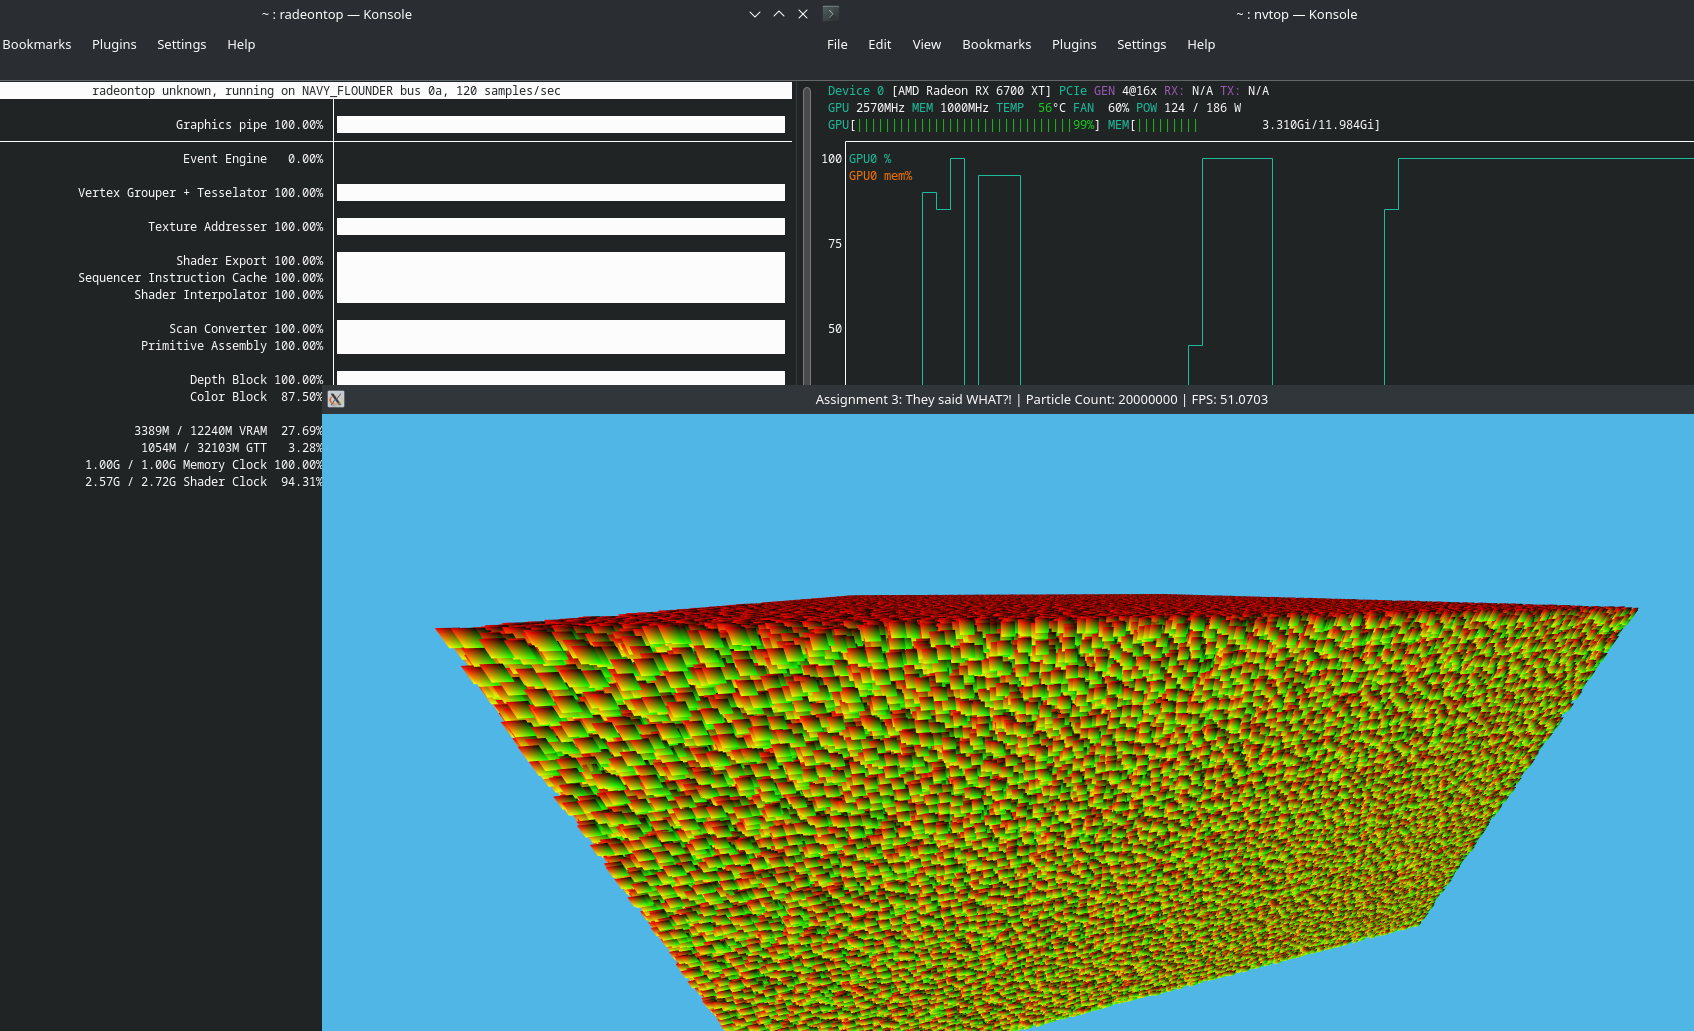
\includegraphics[width=1.6\linewidth]{screenshot002}}
	\caption[]{20 million particles distributed in a 50x25x50 cube with load monitors}
	\label{fig:screenshot002}
\end{figure}

\begin{figure}[H]
	\centerline{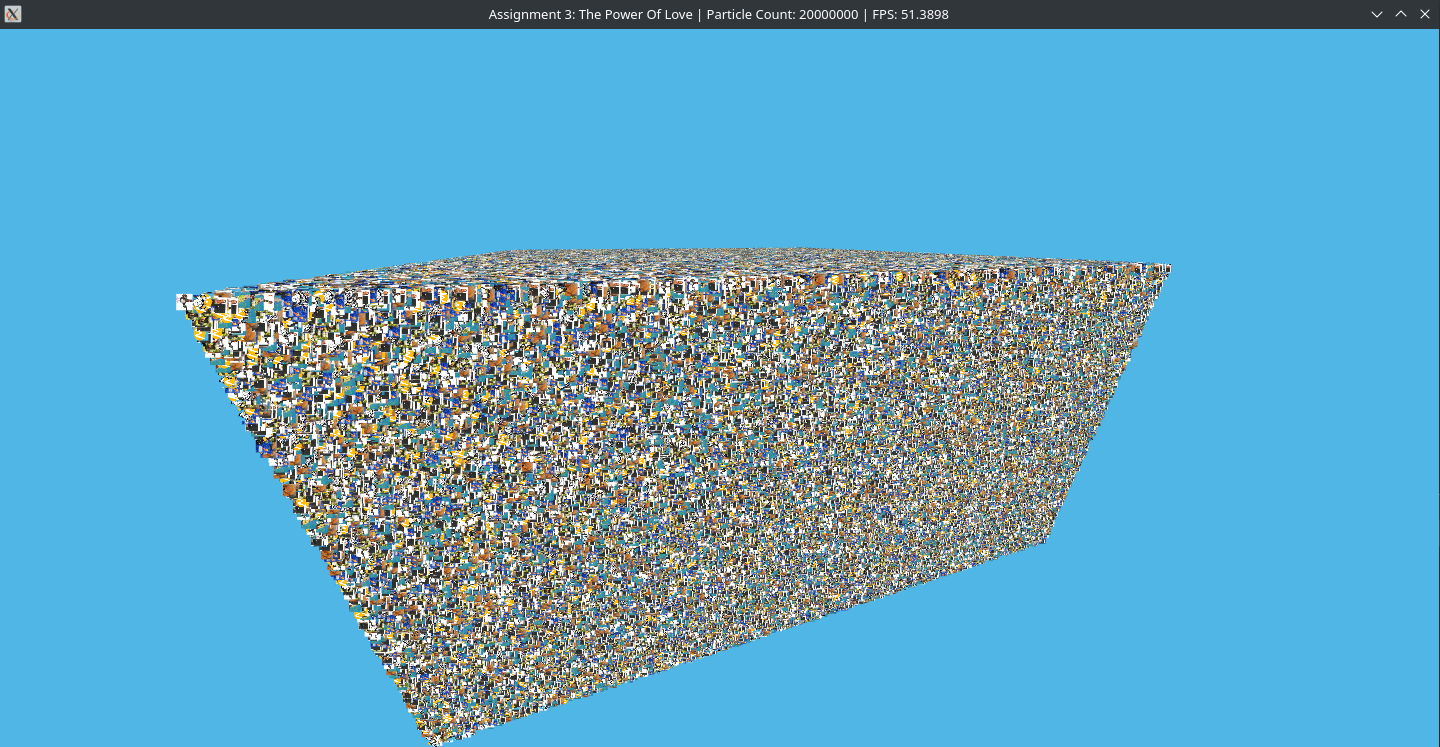
\includegraphics[width=1.6\linewidth]{screenshot003}}
	\caption{20 million particles on the new renderer}
	\label{fig:newrender}
\end{figure}

\begin{figure}
	\centering
	\centerline{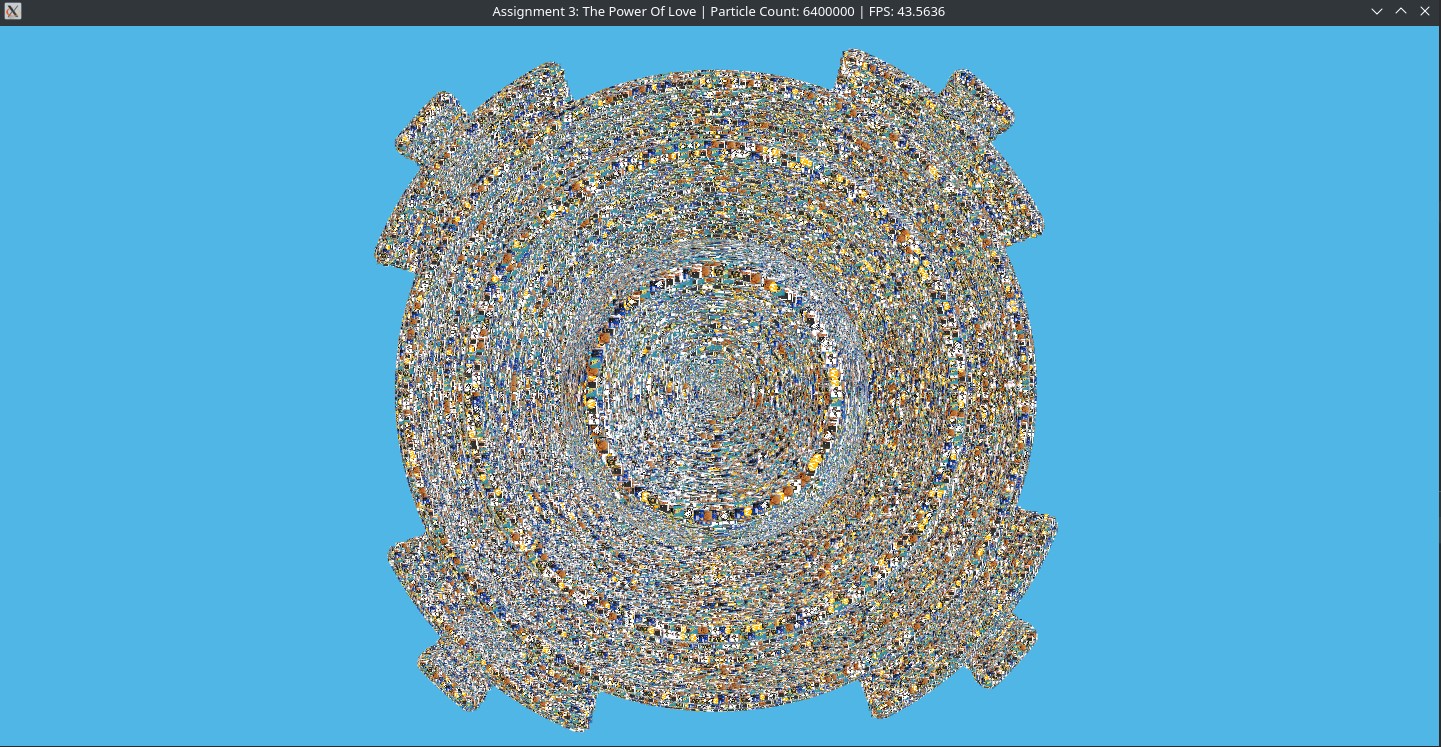
\includegraphics[width=1.6\linewidth]{screenshot004}}
	\caption{6.4 million particles, fillrate (not compute) limited.}
	\label{fig:phyiscsrend}
\end{figure}

\begin{figure}
	\centering
	\centerline{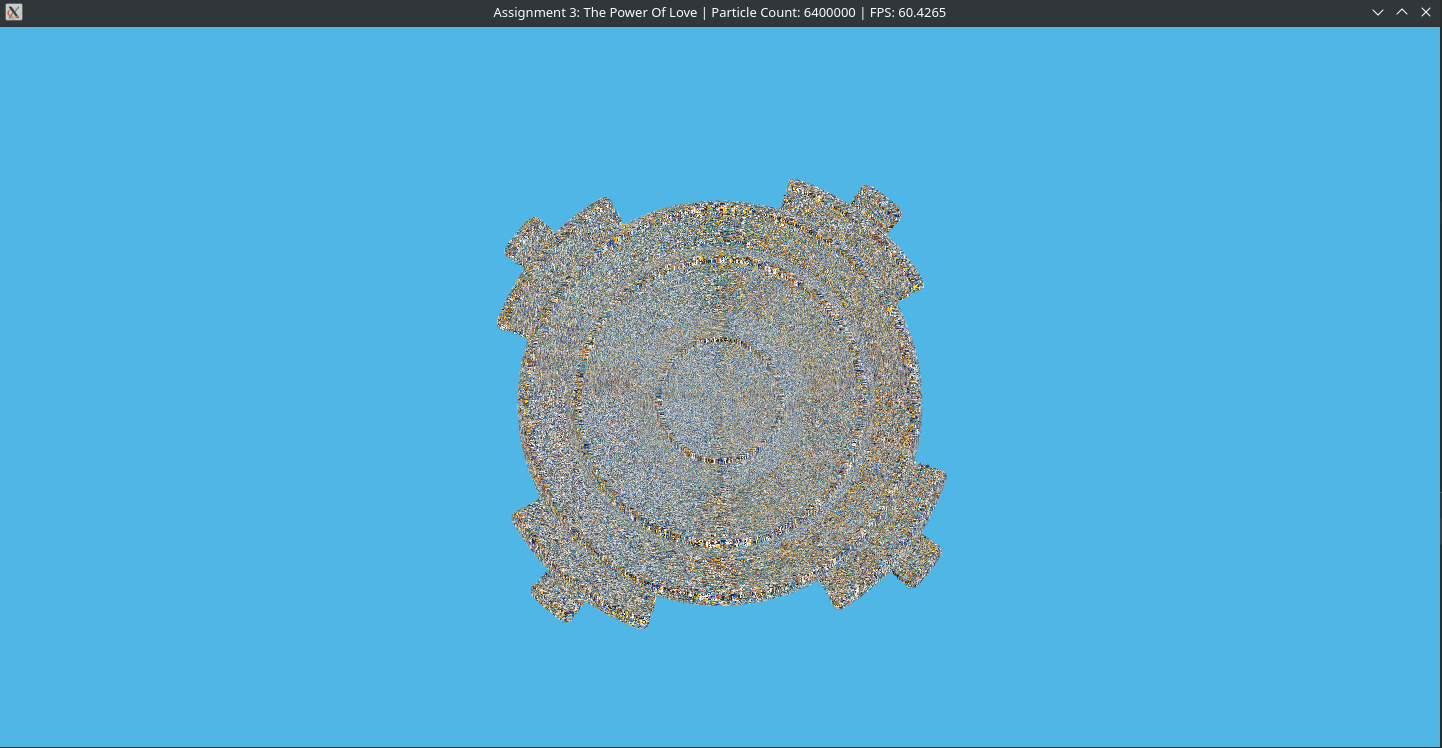
\includegraphics[width=1.6\linewidth]{screenshot005}}
	\caption{6.4 million particles, zoomed out, showing fillrate as the limiting factor in speed.}
	\label{fig:phyiscsrendfill}
\end{figure}



\nocite{*}

\bibliographystyle{plain}
\bibliography{references.bib}

\end{document}          
